\documentclass[11pt,a4paper]{article}

\usepackage[utf8]{inputenc} 
\usepackage[T1]{fontenc} 
\usepackage{lmodern}
\usepackage[margin=2cm]{geometry}
\usepackage[german]{babel}
\usepackage{amsmath} 
\usepackage{graphicx} 
\usepackage{booktabs}
\usepackage{hyperref}
\hypersetup{
    colorlinks,
    citecolor=red,
    filecolor=black,
    linkcolor=black!20!blue!90!,
    urlcolor=black} 
\usepackage{nicefrac}
\usepackage[table]{xcolor}
\usepackage{tocloft}

\setlength{\parindent}{0pt}
\setlength{\parskip}{1ex plus 0.5ex minus 0.5ex}

\definecolor{incolor}{rgb}{0.0, 0.0, 0.5}

\hbadness=99999

\newcommand{\refpy}[1]{Siehe Anhang: \textit{Rechnungen in Python} (\texttt{{\color{incolor}In [{\color{incolor}#1}]}})}
\newcommand\dif{\mathop{}\!\mathrm{d}}
\newcommand{\halftime}[4]{\begin{figure}[h]
\begin{minipage}{.#1\textwidth}#3\end{minipage}\begin{minipage}{.#2\textwidth}
\centering
#4\end{minipage}
\end{figure}}
\renewcommand{\vec}{\boldsymbol}

\begin{document}

% name of experiment
% date of experiment
% name of assistant
{
\centering 
\large 
Physiklabor für Anf\"anger*innen \\
Ferienpraktikum im Sommersemester 2018 \\[4mm]
\textbf{\LARGE 
Versuch 23: Schallwellen
} \\[3mm]
(durchgef\"uhrt am 08.10.2018 bei Pascal Wunderlin) \\
Ye Joon Kim, Patrick M\"unnich\\
\today \\[10mm]
}

\vspace{50pt}
\tableofcontents
\vspace{22pt}
\listoftables
\vspace{22pt}
\listoffigures
\pagebreak

\section{Ziel des Versuchs}
Das Ziel dieses Versuchs ist es, die Schallschallgeschwindigkeit von Luft auf drei Weisen zu bestimmen. 

\section{1. Versuchsteil: Bestimmung der Schallgeschwindigkeit mit einem Quinckeschen Rohr}

\subsection{Theorie}

XXXX

\subsection{Aufbau}

\begin{figure}
	\centering
	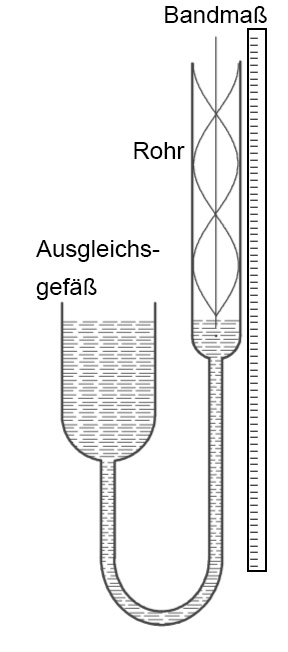
\includegraphics[scale=0.5]{Abb1}
	\caption{Aufbau zum ersten Versuchsteil: Ein quinckeschen Rohr.}
\end{figure}
Für den ersten Versuchsteil wurde ein Quinckesches Resonanzrohr verwendet (Siehe Abbildung 1). 

% describe set up
% insert pic name, designation, toc caption, caption, label
%\halftime{5}{5}{TEXT}{\fbox{\includegraphics[width=0.5\textwidth]{NAME}}
%   \renewcommand\thefigure{BX}
%\caption[XXXX]{XXXX \cite{Anleitung}}
%\label{Pic:X}}

\subsection{Durchführung}
Die Frequenzgenerator und der Oszillator wurden angeschaltet. Es wurde dann ein Frequenz zwischen 2 kHz und 7 kHz ausgewählt. Die Wasserhöhe in dem Rohr wurde dann verkleinert, indem man der Ausgleichsgefäß senkt. Als eine maximale Amplitude in dem Oszilloskop beobachtet wurde, wurde die Höhe des Wasserspiegels in dem Rohr mit einem Maßband gemessen. Dies wurde auch gemessen, als ein Minimum beobachtet wurde. Für jede Frequenz wurden die Wasserhöhe für 8-10 Maximum und Minimum gemessen. Es wurden drei Unterschiedliche Frequenzen untersucht. 


\subsection{Auswertung und Fehleranalyse}

Um mit unseren Messdaten die Schallgeschwindigkeit bestimmen zu k\"onnen, tragen wir zuerst die Lagen der Maxima und Minima in Diagramme auf. Daraufhin f\"uhren wir eine lineare Regression durch und f\"ugen sie dem Bild hinzu. Die Resultierenden Graphiken im Anhang als Abbildung \ref{Abb:3}, \ref{Abb:4} und %\ref{Abb:5} gefunden werden.

Um die lineare Regression durchf\"uhren zu k\"onnen, nehmen wir uns das folgende Polynom ersten Grades vor:
\[ a+bx\]

F\"ur $a$ berechnen wir

\[a=\frac{\sum x_i^2\sum y_i-\sum x_i\sum x_iy_i}{n\sum x_i^2-(\sum x_i)^2}\]
und f\"ur b
\[b=\frac{n\sum x_iy_i-\sum x_i\sum y_i}{n\sum x_i^2-(\sum x_i)^2}.\]

Wollen wir dessen Unsicherheiten bestimmen, so k\"onnen wir die folgenden Formeln verwenden:
\[
s=\sqrt{\frac{1}{n-2}\sum^n_{i=1}[y_i-(a+bx_i)]^2}\]

\[\Delta a=s\sqrt{\frac{\sum x_i^2}{n\sum x_i^2-(\sum x_i)^2}}\]

\[\Delta b=s\sqrt{\frac{n}{n\sum x_i^2-(\sum x_i)^2}}\]

Mit diesen Formeln erhalten wir als Werte

\begin{table}[h]
	\centering
	\begin{tabular*}{0.50\textwidth}{@{\extracolsep{\fill}}cccc}
		\toprule
		Messreihe & $b$ & $u_b$ \\
		& cm & cm\\
		1 & -0.27 & 0.03\\
		2 & -0.27 & 0.03\\
		3 & -0.27 & 0.03\\
		\bottomrule
	\end{tabular*}
\caption{Die berechneten Steigungen der linearen Regressionen von $\nu$ gegen $l$}
\label{Table1}
\end{table}

Wir nutzen dann die Steigung, um die Wellenl\"angen zu bestimmen. Wir berechnen dann einfach mit
\begin{equation}
c=\nu\lambda
\end{equation}
die Ausbreitungsgeschwindigkeit der Wellen. Die Ergebnisse lauten dann:







\section{Diskussion der Ergebnisse}

XXXX

\pagebreak

\section{2. Versuchsteil: Bestimmung der Ultraschallgeschwindigkeit durch die Messung der Wellenlänge.}
\subsection{Theorie}
\subsection{Aufbau}
\begin{figure}
	\centering
	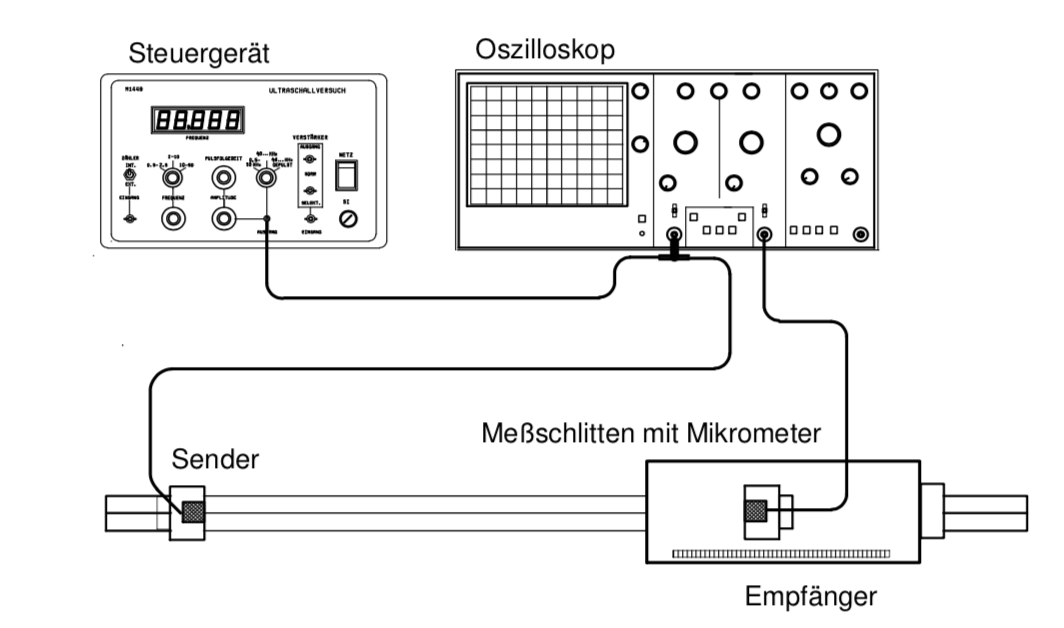
\includegraphics[scale=0.5]{Abb2}
	\caption{Aufbau zum zweiten Versuchsteil}
\end{figure}

Für diesen Versuchsteil wurden ein Ultraschallsender und -empfänger, ein Oszilloskop, ein Signalgenerator und ein Mikrometerschraube (Siehe Abbildung 2). 

\subsection{Durchführung}
Der Sender und der Empfänger (mit dem Mikrometerschraube) wurden auf beiden Seiten der Bank fixiert. Der Oszilloskop wurde angeschaltet und justiert, sodass beide Signale im Bildschirm zu sehen waren. Der Empfänger wurde dann mit dem Mikrometerschraube verschoben, sodass die zwei angezeigten Signalen in Deckung waren. Sein Position relativ zum Mikrometerschraube wurde dann aufgenommen. Der Empfänger wurde dann wiederum mit dem Mikrometerschraube verschoben, bis die zwei Signalen wieder in Deckung waren. Seine Position wurde dann aufgenommen. Die Positionen wurde 10-mal für jedes mal, dass die zwei Signalen in Deckung waren, gemessen. Dieser Prozess wurde für vier verschiedene Startpositionen des Empfängers wiederholt. 



\subsection{Auswertung und Fehleranalyse}
Für jede Messreihe wurde die $x$ Werte gegen $k$ aufgetragen (Siehe Anhang). Die lineare Regressionen wurden mithilfe eines Excel-Dokuments mit den folgenden Formel berechnet: 

Die Steigung $b$ ist:
$$ b = \frac{n\sum k_ix_i-\sum k_i \sum x_i}{n \sum k_i^2 - (\sum k_i)^2}$$

und ihre Unsicherheit:
$$u_b = s\cdot \sqrt{\frac{n}{n\sum k_i^2 - (\sum k_i)^2}}$$
Mit 
$s = \sqrt{\frac{1}{n-2}\sum [x_i-(a+bk_i)]^2}$

Es wurden nur die Steigungen und deren Unsicherheiten berechnet, da der Achsenabschnitt ist irrelevant. Die berechneten Steigungen und deren Unsicherheiten für jede Messreihe sind in Tabelle \ref{Table1} zu sehen. 


\begin{table}[h]
	\centering
	\begin{tabular*}{0.50\textwidth}{@{\extracolsep{\fill}}cccc}
		\toprule
		Messreihe & $b$ & $u_b$ \\
		& cm & cm\\
		1 & 9,1 & 1,7 \\
		2 & 8,6 & 0,2 \\
		3 & 8,46 & 0,15 \\
		4 & 8,51 & 0,02 \\
		\bottomrule
	\end{tabular*}
\caption{Die berechneten Steigungen der linearen Regressionen von $x$ gegen $k$}
\label{Table1}
\end{table}

Um die Schallgeschwindigkeit zu bestimmen wurde die folgende Formel benutzt:
$$ c = \nu\lambda$$

Für $\nu$ wurde die Durchschnittliche Frequenz während der Messreihe benutzt. Seine Unsicherheit wurde mit der Standardunsicherheit berechnet nämlich:
$$ u_\nu = \frac{s_\nu}{\sqrt{n}}$$
und
$$ s_{\bar{\nu}} = \sqrt{\frac{\sum_{i=1}^{n}(\nu_i-\bar{\nu})^2}{n-1}}$$.

Für die Unsicherheiten der Schallgeschwindigkeiten wurde die vereinfachte gaußsche Fehlerfortpflanzung für Produkte benutzt, aber da die Beträge von $\frac{u_\lambda}{\lambda}$ rund 100-mal größer als die von den $\frac{u_\nu}{\nu}$ Terme waren, wurde die Letzteren vernachlässigt. Die Unsicherheit von $c$ ist deshalb:
$$ u_c = \left| \frac{u_\lambda}{\lambda}\right|$$

Die berechnete Werte für die Schallgeschwindigkeiten und ihre Unsicherheiten sind in Tabelle \ref{Table2} zu sehen.

\begin{table}[h]
	\centering
	\begin{tabular*}{0.50\textwidth}{@{\extracolsep{\fill}}cccc}
		\toprule
		Messreihe & $c$ & $u_c$ \\
		& m/s&m/s\\
		1 & 370 & 70 \\
		2 & 350 & 10 \\
		3 & 342 & 6 \\
		4 & 344,2 & 0,8 \\
		\bottomrule
	\end{tabular*}
	\caption{Die berechnete Schallgeschwindigkeit für alle Messreihe}
\label{Table2}
\end{table}

Die $c$ Werte wurden gemittelt und ihre Standardunsicherheit berechnet. 

$$ c = (351 \pm 6) \textrm{ m/s}$$

Die Unsicherheit wurde genau wie oben mit
$$u_{\bar{c}} = \frac{1}{\sqrt{n}} \sqrt{\frac{\sum_{i=1}^{n}(c_i-\bar{c})^2}{n-1}}$$
berechnet. 




\subsection{Diskussion der Ergebnisse}


Die mit der Wellenlängemessung bestimmte Schallgeschwindigkeit ist:
$$ c = (361 \pm 6) \textrm{m/s} $$

Um zu sehen ob dieses Ergebnis und der theoretischer Wert miteinander verträglich sind wurde ihre Differenz in Einheiten der Standardunsicherheit berechnet, nämlich mit:
$$ t = \frac{c - c_\textrm{theo}}{s_{\bar{c}}} $$
, was $t \approx 1,03 $ beträgt. 
	
Da dieser Wert kleiner als 2 ist, sind die zwei Werte miteinander verträglich, und da die relative Unsicherheit 1,7\% ist dieses Ergebnis auch signifikant. 


\section{3. Versuchsteil: Bestimmung der Ultraschallgeschwindigkeit durch die Messung der Laufzeit}

\subsection{Theorie}
\subsection{Aufbau}
\begin{figure}[h]
	\centering
	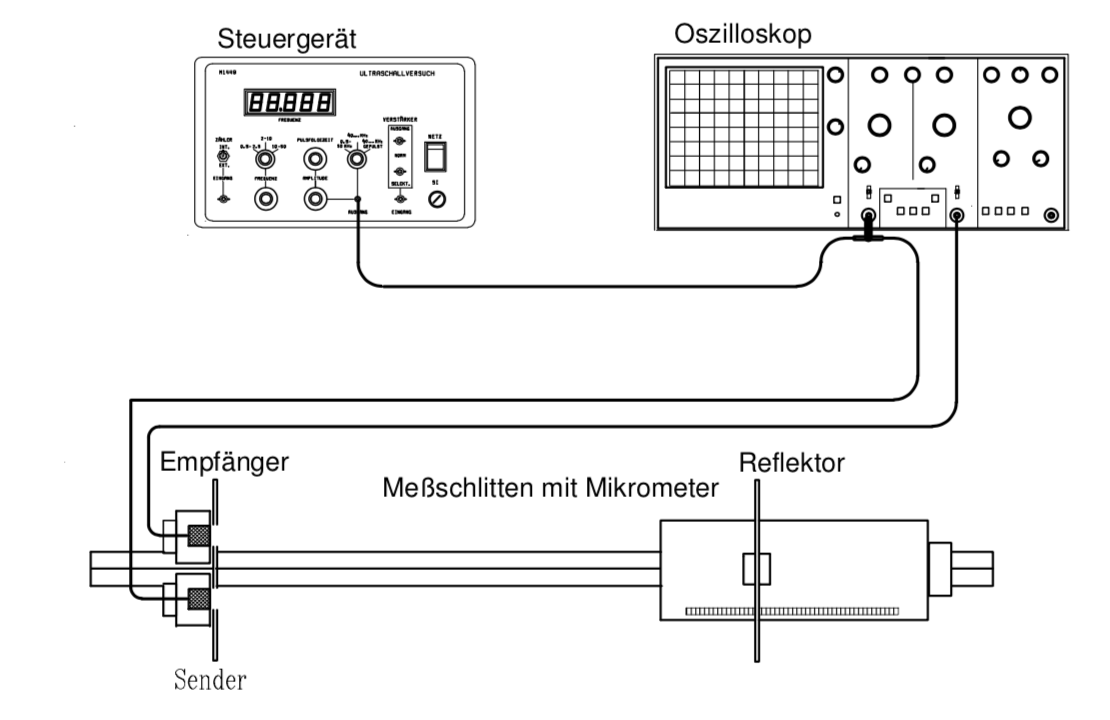
\includegraphics[scale=0.5]{Abb3}
	\caption{Aufbau zum dritten Versuchsteil}
\end{figure}
Für diesem Versuchsteil wurden dieselben Apparate wie in dem zweiten Teil und ein Reflektor benutzt (Siehe Abbildung 3). 

\subsection{Durchführung}
Zu diesem Versuchsteil wurde der Empfänger und der Sender auf derselben Seite der Bank fixiert. Auf der anderen Seite wurde ein Reflektor installiert. Es wurde die Betriebsart 3 des Frequenzgenerators ausgewählt. Der Oszilloskop und Frequenzgenerator wurden angeschaltet und justiert, sodass zwei Pulse im Bildschirm des Oszilloskops zu sehen waren. Der Abstand zwischen dem Empfänger-Sender Komplex und dem Reflektor wurde mit einem Maßband gemessen. Der Zeitdauer zwischen dem ausgesandten Puls und empfangenen Puls wurde direkt mithilfe der Skala auf dem Oszilloskop gemessen. 

\section{Anhang: Tabellen und Diagramme}

\begin{table}[h]
\centering
\caption{XXXX} \vspace{11pt}
$\begin{array}{l}
\textrm{Unsicherheiten:}\\
\textrm{XXXX: } \pm XX \textrm{XX}\\
\end{array}$
\begin{tabular}{ccc}
\toprule
\textrm{XXXX}/\textrm{XX} & \textrm{XXXX}/\textrm{XX} & \textrm{XXXX}/\textrm{XX} \\
\midrule 
2 & 0.26 & 0.23\\
\hline
4 & 0.33 & 0.25\\
\hline 
5 & & 0.3\\
\hline 
6 & 1.25 & 0.83\\
\hline 
8 & 3.9 & 0.83\\ 
\hline
9 & 4.75 & 4.6\\ 
\hline
10 & 4.7 &\\ 
\bottomrule
\end{tabular}
\phantom{$\begin{array}{l}
\textrm{Unsicherheiten:}\\
\textrm{XXXX: } \pm XX \textrm{XX}\\
\end{array}$}
\label{Tab:X}
\end{table}

\begin{figure}[p]
\centering
\fbox{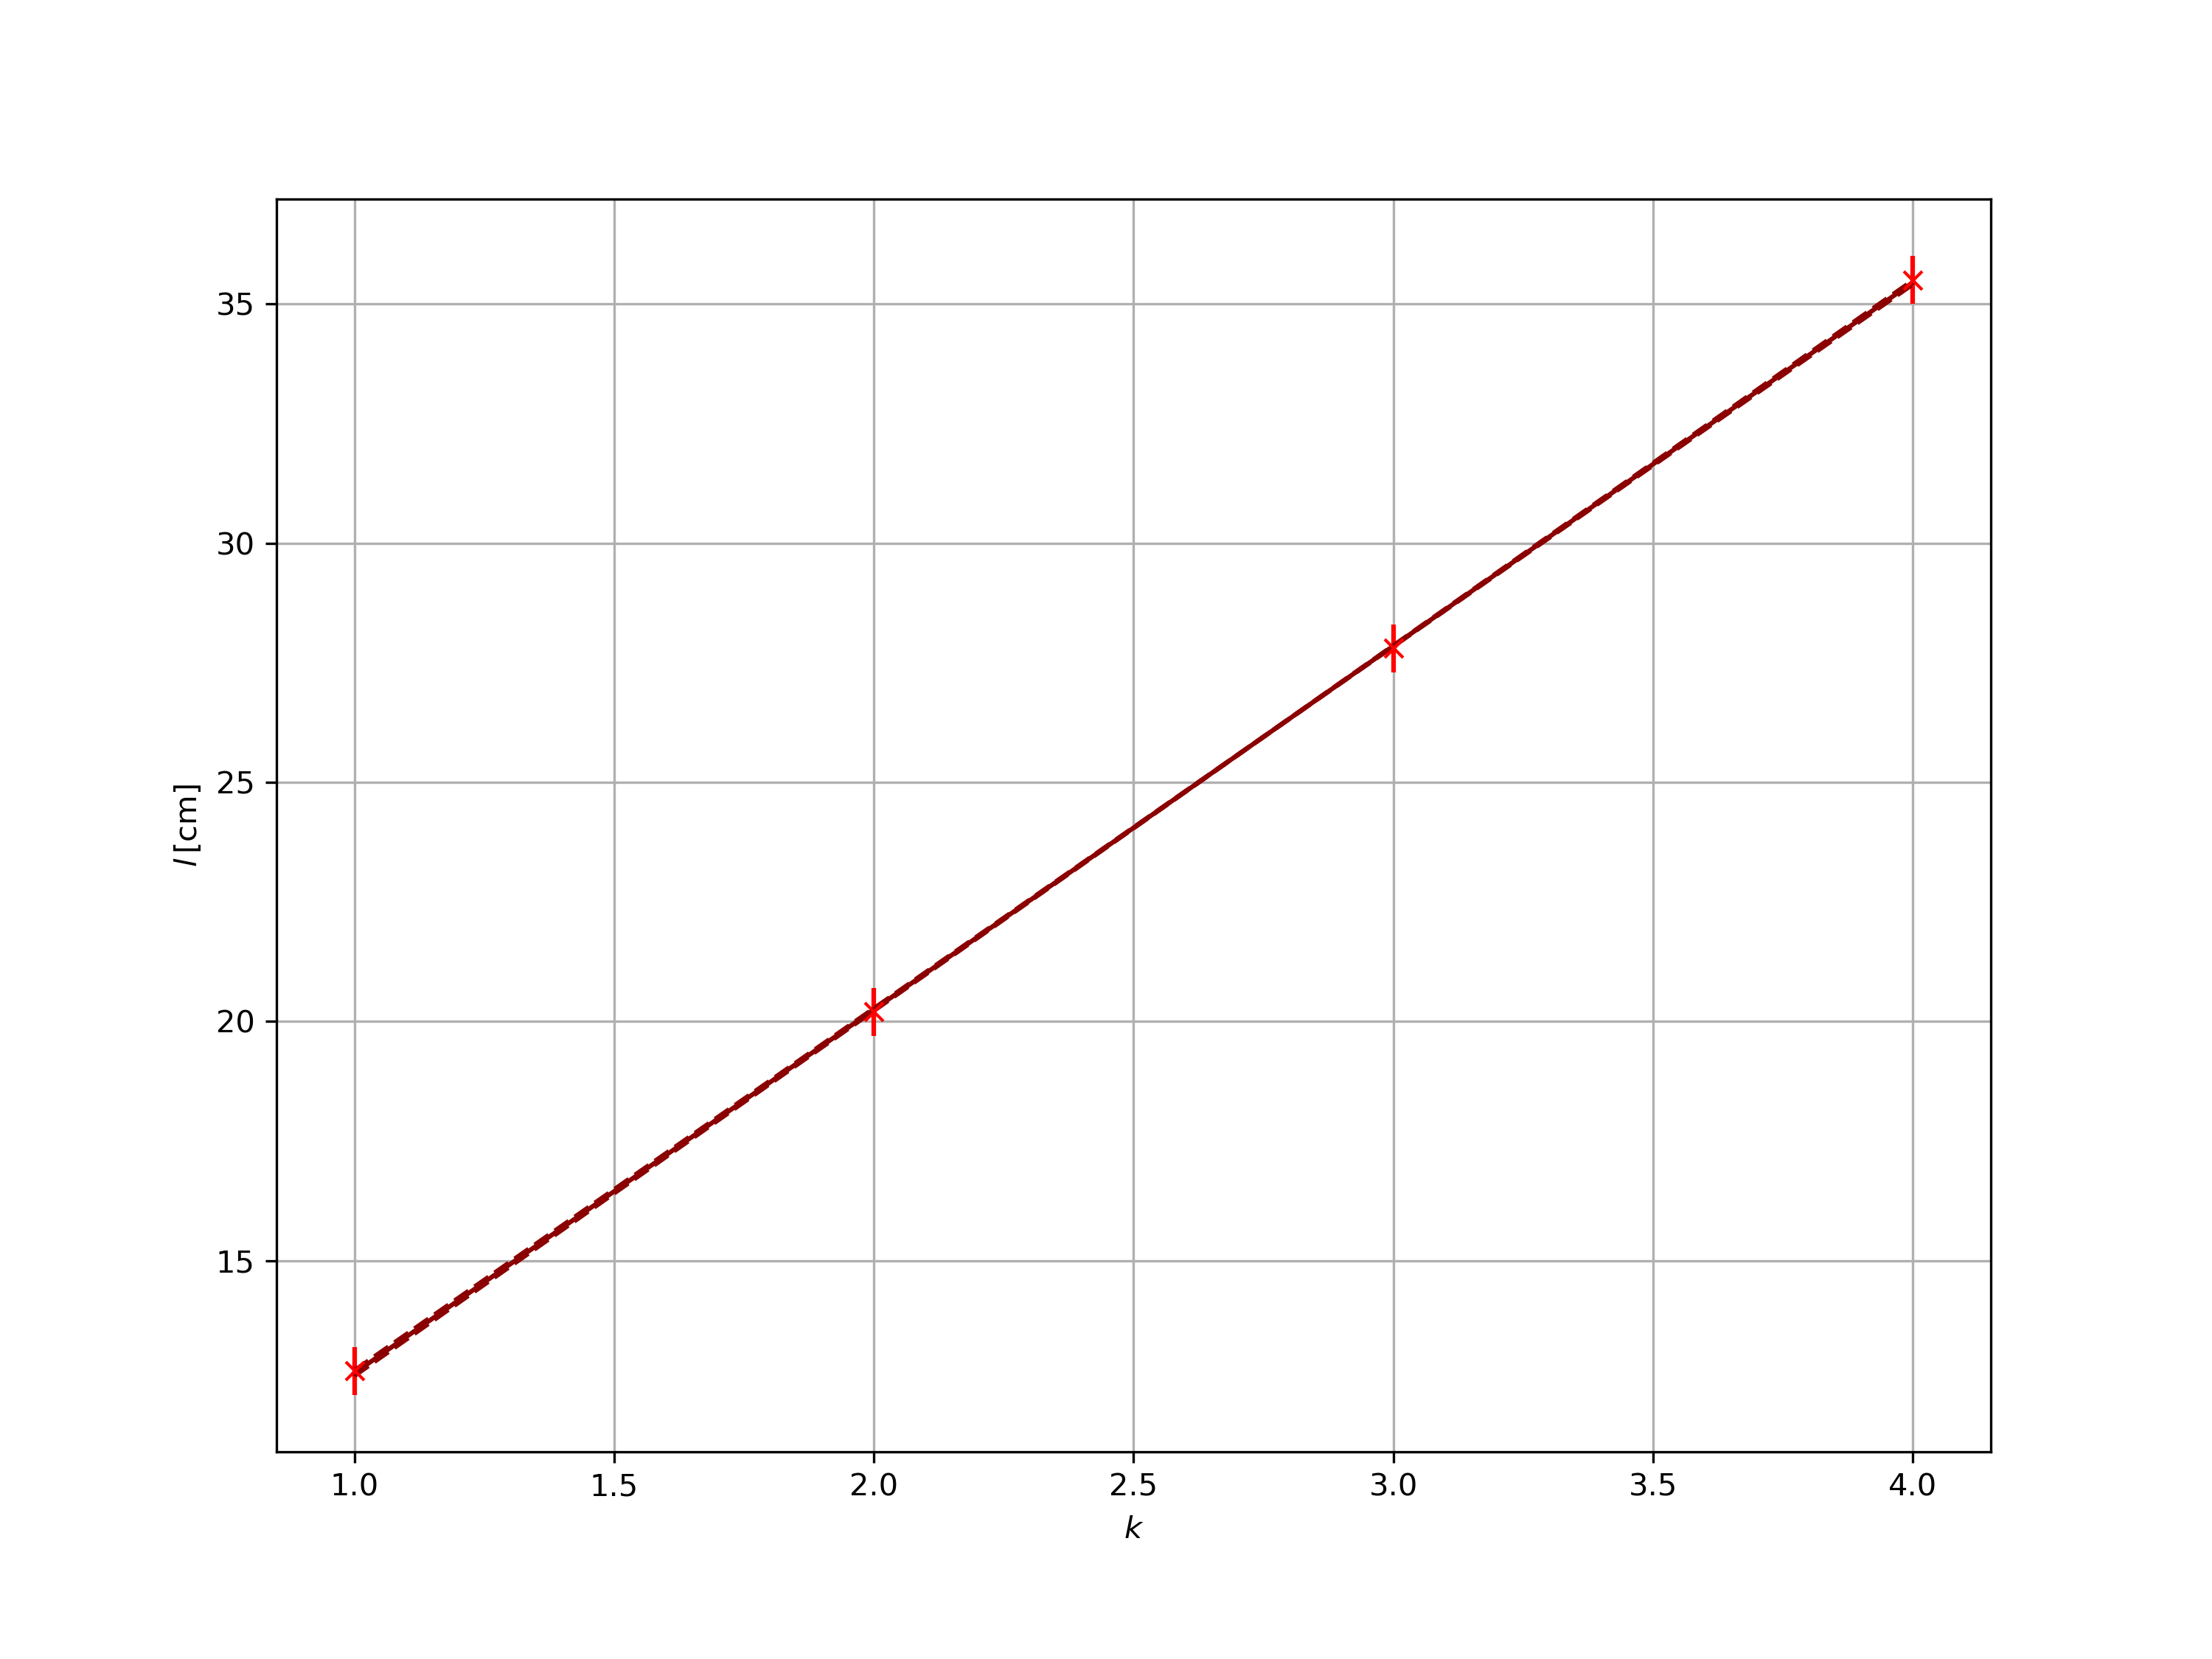
\includegraphics[width=0.8\textwidth]{1minimumonnly}}
\renewcommand\thefigure{3}
\caption[Auftragen der Minima in Abh\"angikeit der Frequenz f\"ur den ersten Versuchsteil]{Auftragen der Minima in Abh\"angikeit der Frequenz f\"ur den ersten Versuchsteil}
\label{Abb:3}
\end{figure}

\begin{figure}[p]
\centering
\fbox{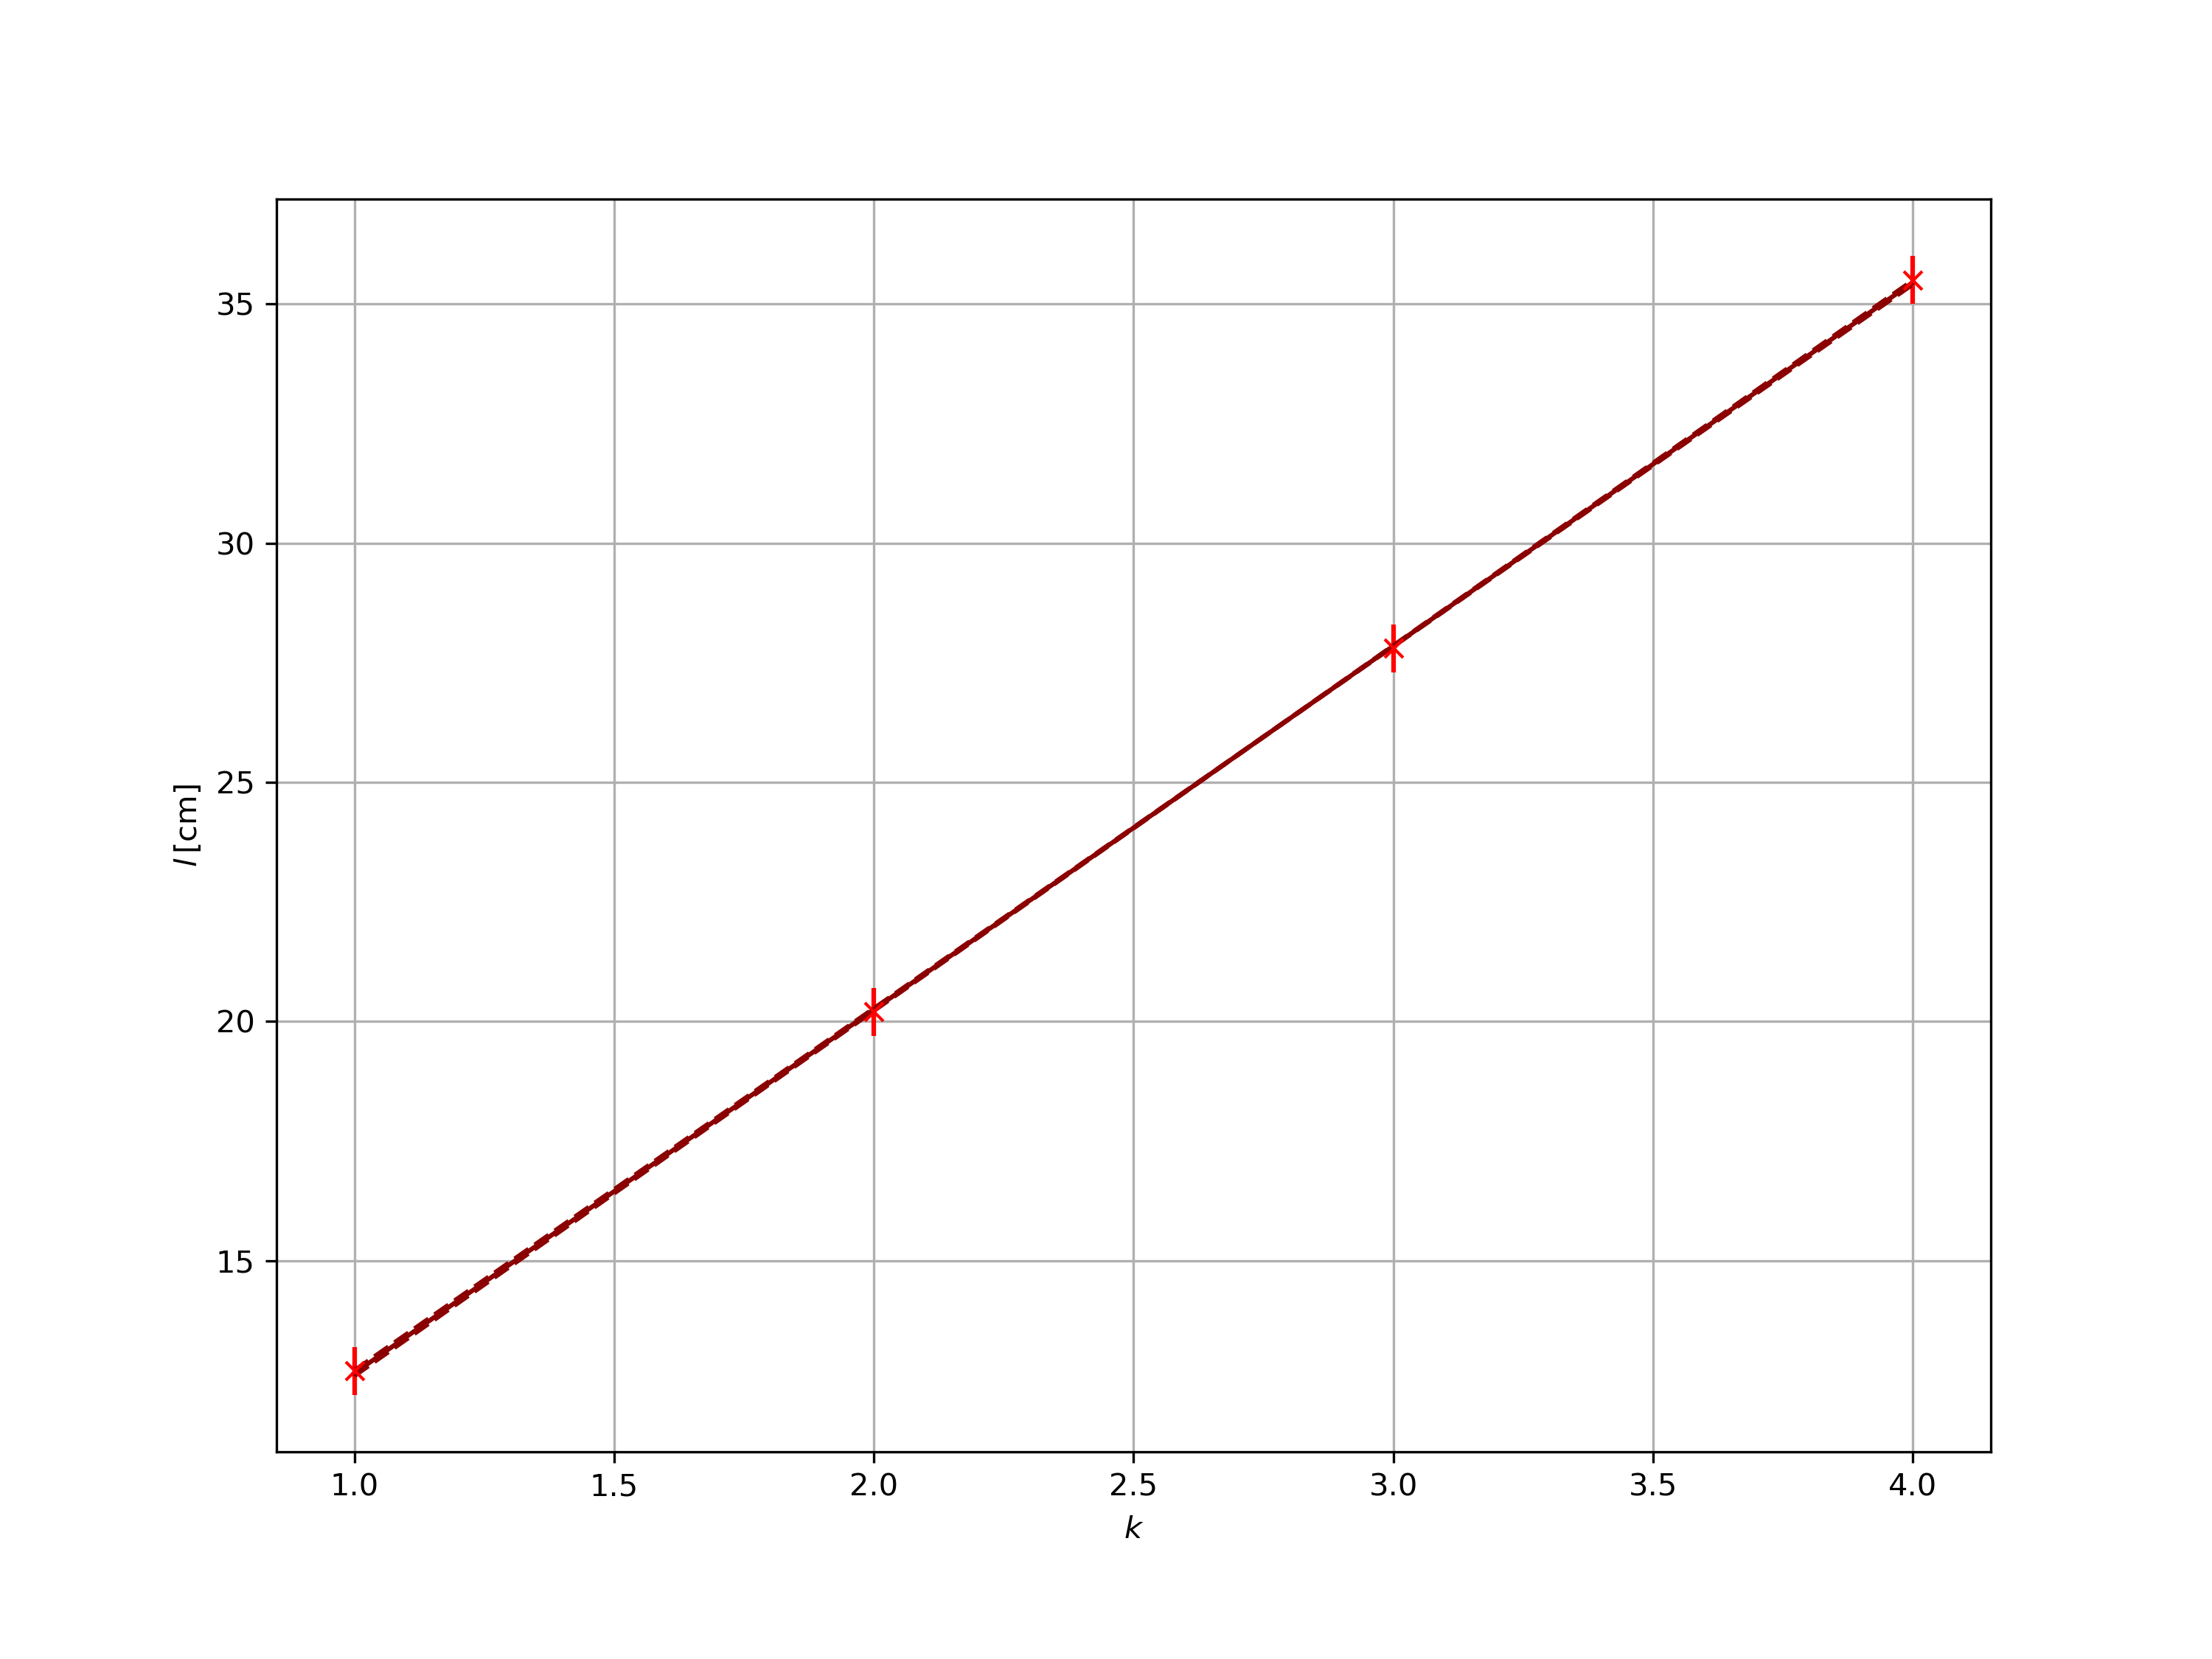
\includegraphics[width=0.8\textwidth]{1minimumonnly}}
\renewcommand\thefigure{3}
\caption[Auftragen der Maxima und Minima in Abh\"angikeit der Frequenz f\"ur den ersten Versuchsteil bei Frequenz um 5036 Hz]{Auftragen der Maxima und Minima in Abh\"angikeit der Frequenz f\"ur den ersten Versuchsteil bei Frequenz um 5036 Hz}
\label{Abb:4}
\end{figure}

\begin{thebibliography}{9}
\bibitem{Uncertainties}''Correlations between variables are automatically handled, which sets this module apart from many existing error propagation codes.'' - https://pythonhosted.org/uncertainties/
\bibitem{Anleitung} Physikalisches Institut der Albert-Ludwigs-Universität Freiburg (Hrsg.) (08/2018): Versuchsanleitungen zum Physiklabor für Anfänger*innen, Teil 1, Ferienpraktikum im Sommersemester 2018.
\end{thebibliography}

\end{document}